% !TeX root = ../../../main.tex
\subsubsection{Synthetic Experiment Results and Analyses}\label{ch04:sec:synth_results}


We begin with synthetic datasets, where we evaluate 53 estimator variants across the 40 synthetic datasets (Section~\ref{ch04:sec:bench}), systematically spanning varying causal configurations and survival scenarios.
This controlled setting enables us to probe estimator robustness under systematic violations of identification assumptions. 
Our analyses aim to address four questions:  
\textbf{(Q1)} Which estimators perform best overall in terms of CATE RMSE and ATE bias?  
\textbf{(Q2)} How do violations of causal assumptions (ignorability, positivity, ignorable censoring) affect performance?  
\textbf{(Q3)} How does the censoring rate influence estimation quality?  
\textbf{(Q4)} How do component choices (imputation algorithms and base learners) affect final CATE accuracy?
% \textbf{(Q4)} For outcome imputation methods, how important is the imputation algorithm?  
% \textbf{(Q5)} How do choices of imputation method and base learner shape final CATE estimates? 


% !TeX root = ../../../main.tex
\begin{figure}[htbp]
\ChFourFloatContents{ch04:fig:average_rank_all}{\caption{(top) Borda count rankings of the top 10 estimator variants (out of 53 total), based on CATE RMSE across 40 datasets and averaged over 10 repeats (lower is better). 
    (bottom) Family-level rankings, where for each dataset the best method variant within each method family is chosen using validation performance and then ranked on the held-out test set.
        \ChFourRebuttal{Black bands connect methods without statistically significant differences (Wilcoxon signed-rank test, FDR-corrected at $\alpha=0.05$). Shaded regions indicate the standard error of the rank across datasets.}
    }}{
    \centering
    
    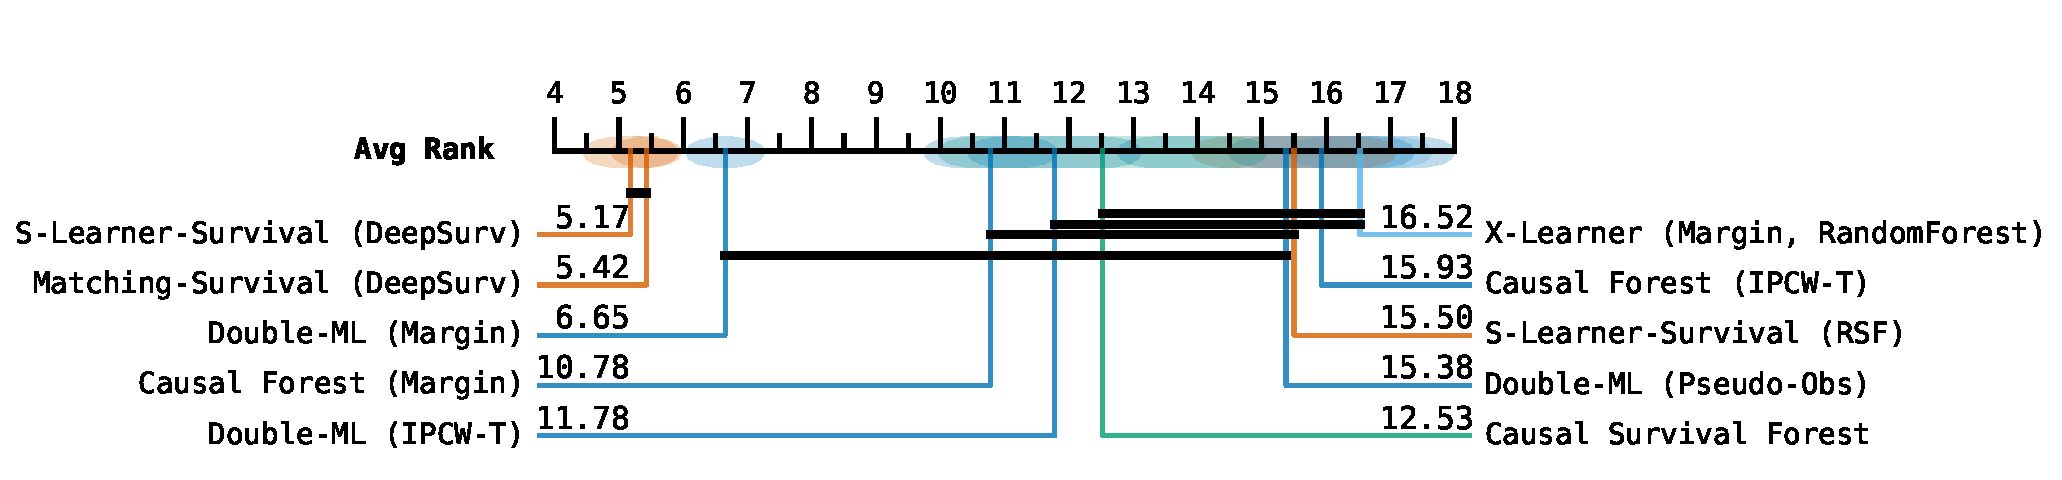
\includegraphics[width=\linewidth]{Chapters/chapter-04/images/figure_results_updated/average_ranks/average_ranking_visualization_method_combination_top_10_total.pdf}
    
    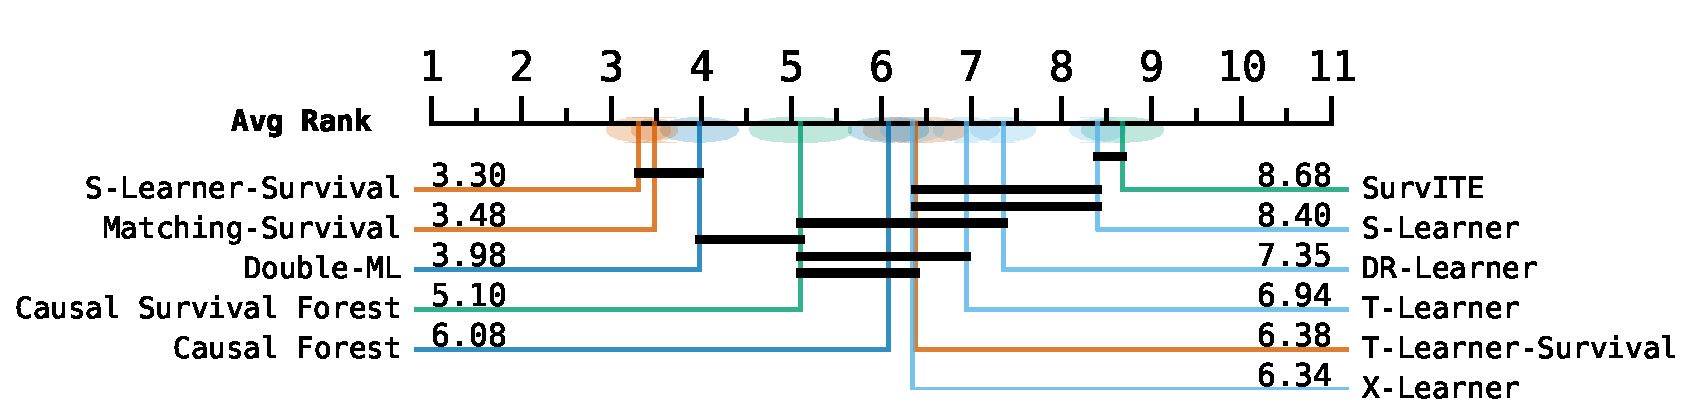
\includegraphics[width=0.83\linewidth]{Chapters/chapter-04/images/figure_results_updated/average_ranks/average_ranking_visualization_method_combination_each_abstract_method.pdf}
    
     
}
\end{figure}


\textbf{Evaluation protocol.}
For each synthetic dataset, we conduct experiments with a random selection of 5,000, 2,500, and 2,500 points for training, validation, and testing samples, repeated over 10 random splits.
The validation set is used for selecting the best variant within each method family, while test sets are reserved strictly for evaluation.
Additional convergence analyses with varying training set sizes are in Appendix~\ref{ch04:app:varying-train-size}.
Across all experiments, the horizon parameter $h$ is set to the maximum observed time in each dataset, which is a common practice that allows for consistent estimation of the RMST over the entire observed period.
Further experimental details, including hyperparameters, are in Appendix~\ref{ch04:app:method_settings}.

We present results using the following visualizations: 
\begin{itemize}
    \item \textbf{Borda count rankings.} {To provide a clear summary across the diverse experimental settings, we adopt the Borda count method, which ranks methods by CATE RMSE in each dataset (lower is better) and then averages the ranks across datasets. This approach yields a single, interpretable score that reflects overall relative performance while accounting for variability across scenarios. Similar strategies have been used in other benchmarking studies (e.g., \citealt{han2022adbench}) to enable transparent comparisons across heterogeneous tasks. We report rankings at two levels: (i) individual estimator variants (\ChFourRebuttal{53} total; Figure~\ref{ch04:fig:average_rank_all}, top), and (ii) aggregated method families, where the best variant per family is selected on validation data (\ChFourRebuttal{11} total; Figure~\ref{ch04:fig:average_rank_all}, bottom). The latter mimics a practical deployment setting where practitioners would tune and select the strongest model within a family. More granular rankings stratified by survival scenario (Figure~\ref{ch04:fig:average_rank_per_scenario}) and by causal configuration (Figure~\ref{ch04:fig:average_rank_per_experiments}) are provided in Appendix~\ref{ch04:app:more-avg-rank}.}
    
    \item \textbf{CATE RMSE.} We report absolute CATE RMSE across 10 repeats, grouped by survival scenario, with one panel per set of eight causal configurations.
In the main paper, we show Scenario \texttt{C} as an illustrative example (Figure~\ref{ch04:fig:cate_mse_scenario_C_main}); results for the other scenarios are deferred to Appendix~\ref{ch04:app:more-cate-mse-plots}.

    \item \textbf{ATE bias.} We report ATE bias results, computed analogously to CATE RMSE, in Appendix~\ref{ch04:app:more-ate-plots}.
While the focus of this benchmark is on CATE estimation, these serve as a complementary check.

    \item \ChFourRebuttal{\textbf{Win-rate analyses.} Complementing the Borda rankings, we also report win-rates that quantify how often each method family attains Top-1, Top-3, and Top-5 performance according to CATE RMSE and ATE bias across all synthetic experiments in Appendix~\ref{ch04:app:additional_synthetic_exps}. Overall win-rates aggregated over all survival scenarios and causal configurations are summarized in Table~\ref{ch04:tab:overall-winrate}, while scenario-specific and configuration-specific win-rates are reported in Tables~\ref{ch04:tab:scenario-winrates},~\ref{ch04:tab:winrate-rct-configs}, and~\ref{ch04:tab:winrate-obs-configs}. These summaries highlight not only which methods perform well on average, but also which ones most consistently appear among the top performers under varying censoring regimes and patterns of causal-assumption violations.}
\end{itemize}
Additionally, in Appendix~\ref{ch04:app:auxiliary-eval-results}, we report a series of auxiliary evaluations of key components, including imputation error (Appendix~\ref{ch04:subapp:impute-eval}) for imputation-based methods and regression model accuracy (Appendix~\ref{ch04:subapp:base-reg-eval}) or survival model performance (Appendix~\ref{ch04:subapp:base-surv-eval}) for meta-learners.
These results establish how component-level performance relates to downstream CATE estimation.

% We compute method rankings using the Borda count method, where methods are ranked by their CATE RMSE performance in each experimental setting (lower RMSE means better rank), and the resulting ranks are averaged across all settings. Figure~\ref{ch04:fig:average_rank_all} shows rankings from two different perspectives: specific method configurations (top) and method families (bottom). Detailed rankings within each survival scenario (Figure~\ref{ch04:fig:average_rank_per_scenario}) and causal configuration (Figure~\ref{ch04:fig:average_rank_per_experiments}) are provided in Appendix~\ref{ch04:app:more-avg-rank}, revealing how different approaches perform under specific modeling assumptions and violations. CATE RMSE results for Scenario \texttt{C} are presented in Figure~\ref{ch04:fig:cate_mse_scenario_C_main}, with results for other scenarios and ATE bias analyses in Appendix~\ref{ch04:app:more-cate-mse-plots} and \ref{ch04:app:more-ate-plots}.


\setlength{\tabcolsep}{2pt}

% !TeX root = ../../../main.tex
\begin{figure}[htbp]
\ChFourFloatContents{ch04:fig:cate_mse_scenario_C_main}{\caption{CATE RMSE in Scenario \texttt{C} across 10 experimental repeats.}}{
    \centering
    \makebox[\textwidth][c]{
    \begin{tabular}{@{}cc@{}}
        \subfloat[{RCT:\ChFourGrayCheck (50\%), Ignorability:\ChFourGrayCheck, Positivity:\ChFourGrayCheck, Ignorable Censoring:\ChFourGrayCheck}]{\begin{minipage}[t]{0.495\textwidth}
            \centering
            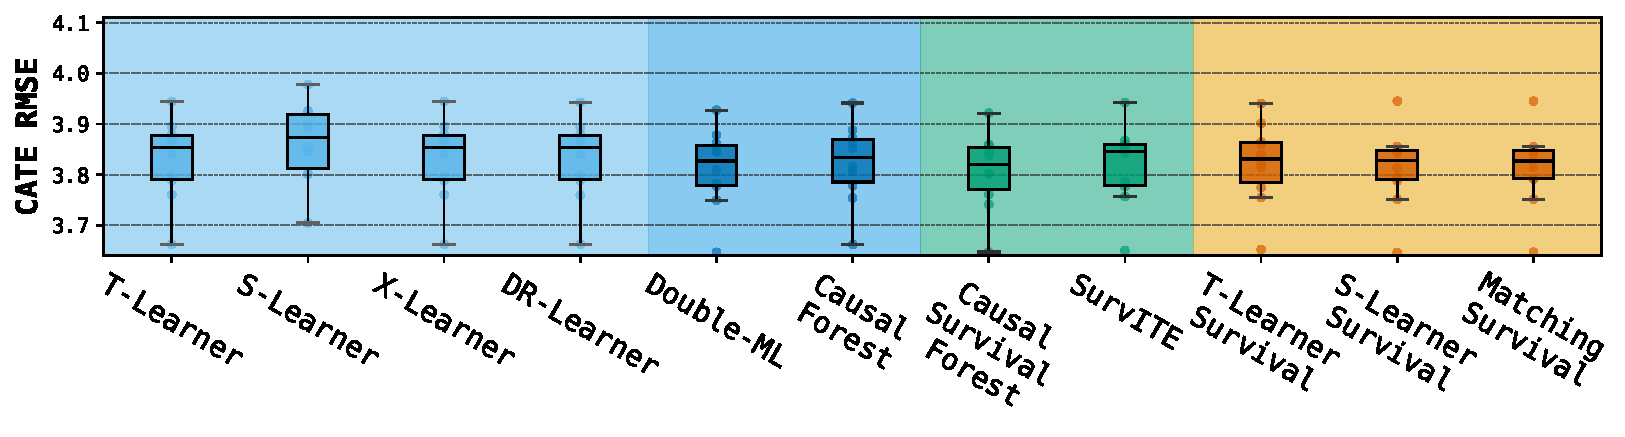
\includegraphics[width=\linewidth]{Chapters/chapter-04/images/figure_results_updated/cate_rmse/Scenario_C_RCT-50_cate_mse.pdf}
            
            \label{ch04:fig:cate_rmse_scenario_C_RCT_50}
        \end{minipage}} &
        \subfloat[{RCT:\ChFourGrayCheck (5\%), Ignorability:\ChFourGrayCheck, Positivity:\ChFourGrayCheck, Ignorable Censoring:\ChFourGrayCheck}]{\begin{minipage}[t]{0.495\textwidth}
            \centering
            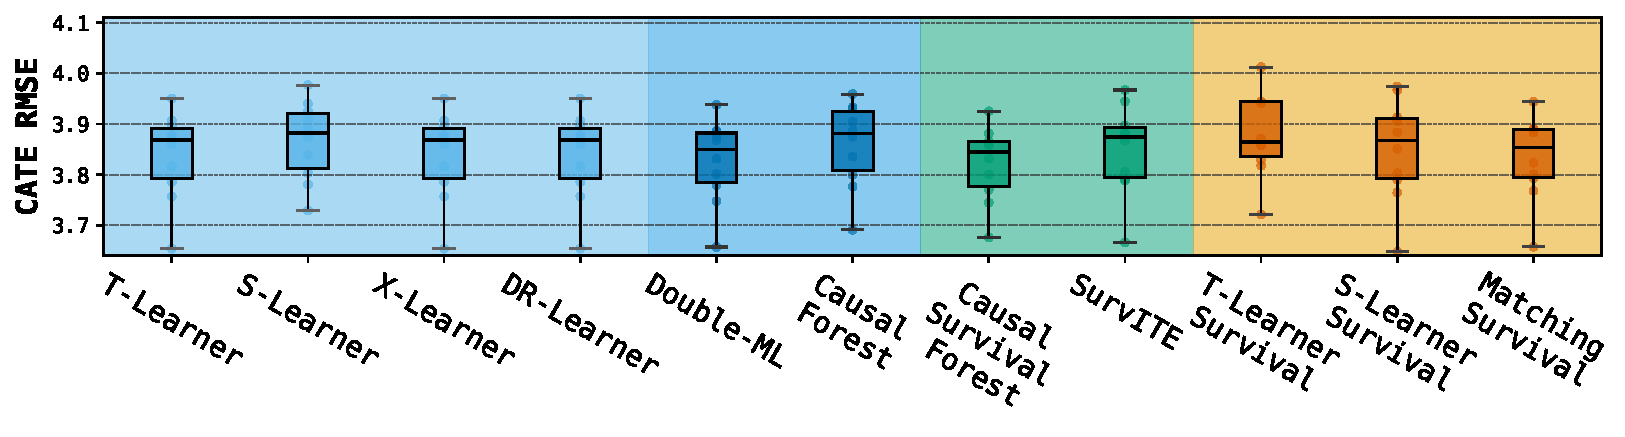
\includegraphics[width=\linewidth]{Chapters/chapter-04/images/figure_results_updated/cate_rmse/Scenario_C_RCT-5_cate_mse.pdf}
            
            \label{ch04:fig:cate_rmse_scenario_C_RCT_05}
        \end{minipage}} \\[1em]
        \subfloat[{RCT:\ChFourBlackCross, Ignorability:\ChFourGrayCheck, Positivity:\ChFourGrayCheck, Ignorable Censoring:\ChFourGrayCheck}]{\begin{minipage}[t]{0.495\textwidth}
            \centering
            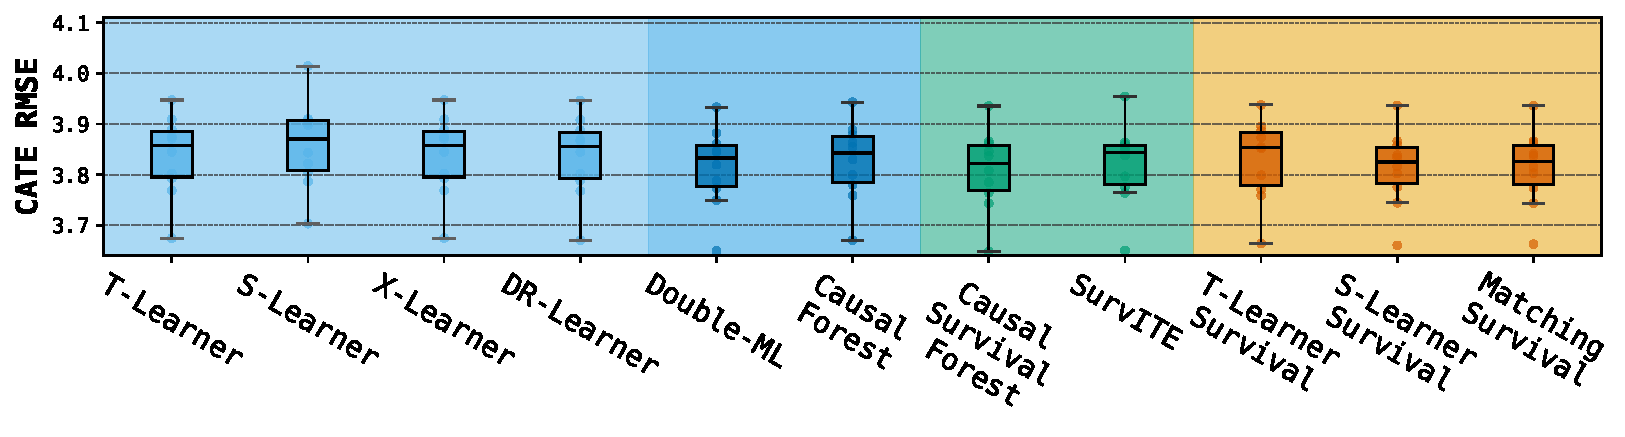
\includegraphics[width=\linewidth]{Chapters/chapter-04/images/figure_results_updated/cate_rmse/Scenario_C_OBS-CPS_cate_mse.pdf}
            
            \label{ch04:fig:cate_rmse_scenario_C_OBS_CPS}
        \end{minipage}} &
        \subfloat[{RCT:\ChFourBlackCross, Ignorability:\ChFourBlackCross, Positivity:\ChFourGrayCheck, Ignorable Censoring:\ChFourGrayCheck}]{\begin{minipage}[t]{0.495\textwidth}
            \centering
            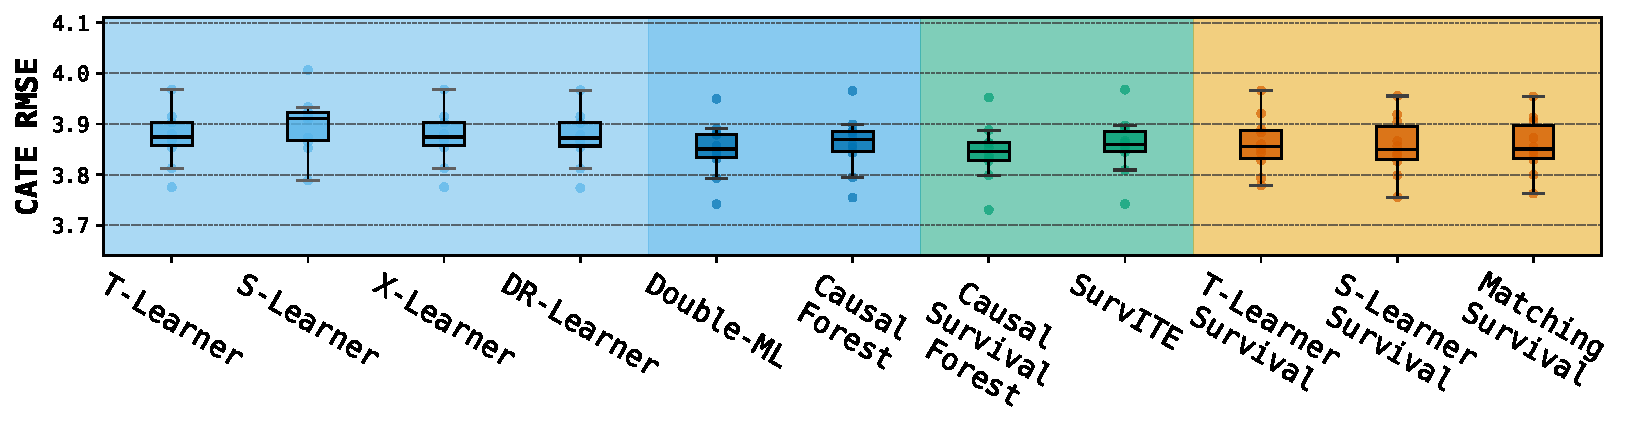
\includegraphics[width=\linewidth]{Chapters/chapter-04/images/figure_results_updated/cate_rmse/Scenario_C_OBS-UConf_cate_mse.pdf}
            
            \label{ch04:fig:cate_rmse_scenario_C_OBS_UConf}
        \end{minipage}} \\[1em]
        \subfloat[{RCT:\ChFourBlackCross, Ignorability:\ChFourGrayCheck, Positivity:\ChFourBlackCross, Ignorable Censoring:\ChFourGrayCheck}]{\begin{minipage}[t]{0.495\textwidth}
            \centering
            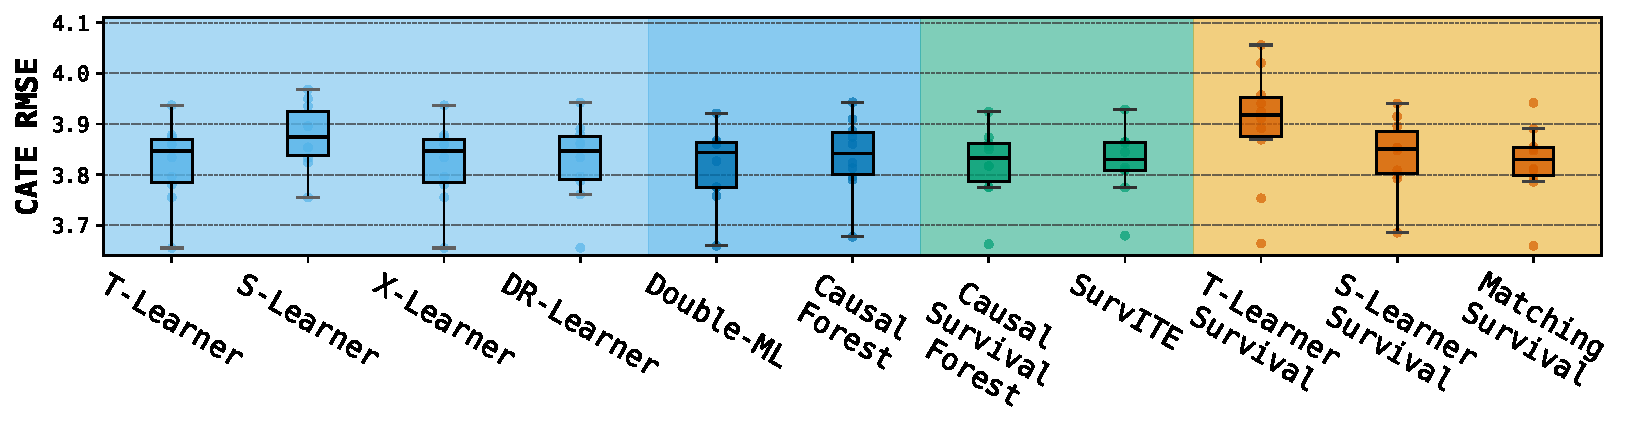
\includegraphics[width=\linewidth]{Chapters/chapter-04/images/figure_results_updated/cate_rmse/Scenario_C_OBS-NoPos_cate_mse.pdf}
            
            \label{ch04:fig:cate_rmse_scenario_C_OBS_NoPos}
        \end{minipage}} &
        \subfloat[{RCT:\ChFourBlackCross, Ignorability:\ChFourGrayCheck, Positivity:\ChFourGrayCheck, Ignorable Censoring:\ChFourBlackCross}]{\begin{minipage}[t]{0.495\textwidth}
            \centering
            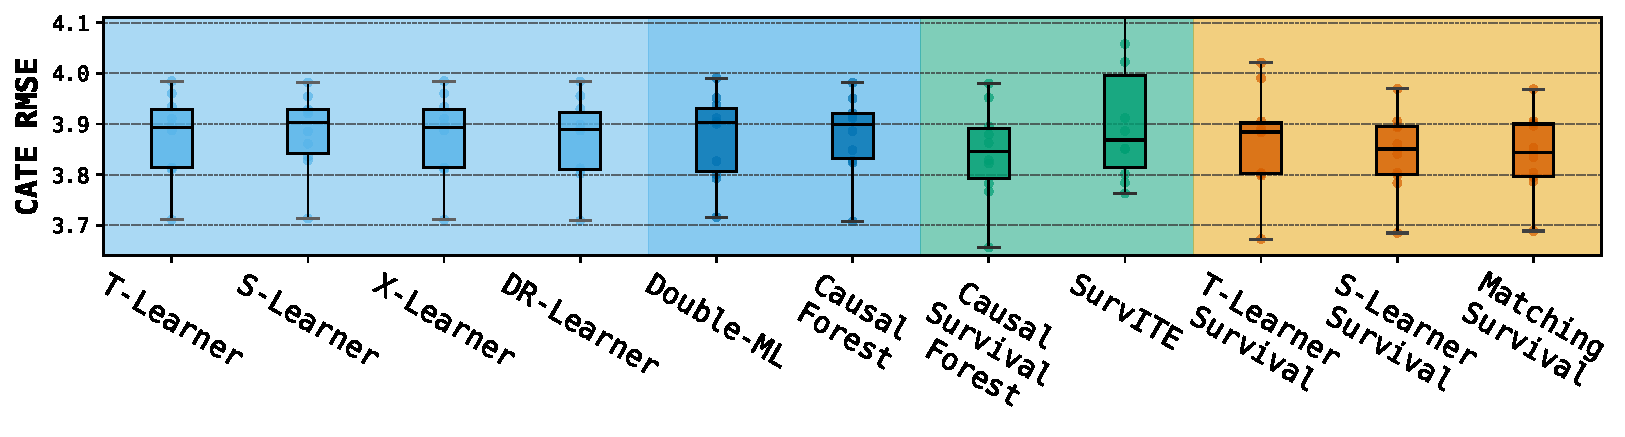
\includegraphics[width=\linewidth]{Chapters/chapter-04/images/figure_results_updated/cate_rmse/Scenario_C_OBS-CPS-IC_cate_mse.pdf}
            
            \label{ch04:fig:cate_rmse_scenario_C_OBS_CPS_InfC}
        \end{minipage}} \\[1em]
        \subfloat[{RCT:\ChFourBlackCross, Ignorability:\ChFourBlackCross, Positivity:\ChFourGrayCheck, Ignorable Censoring:\ChFourBlackCross}]{\begin{minipage}[t]{0.495\textwidth}
            \centering
            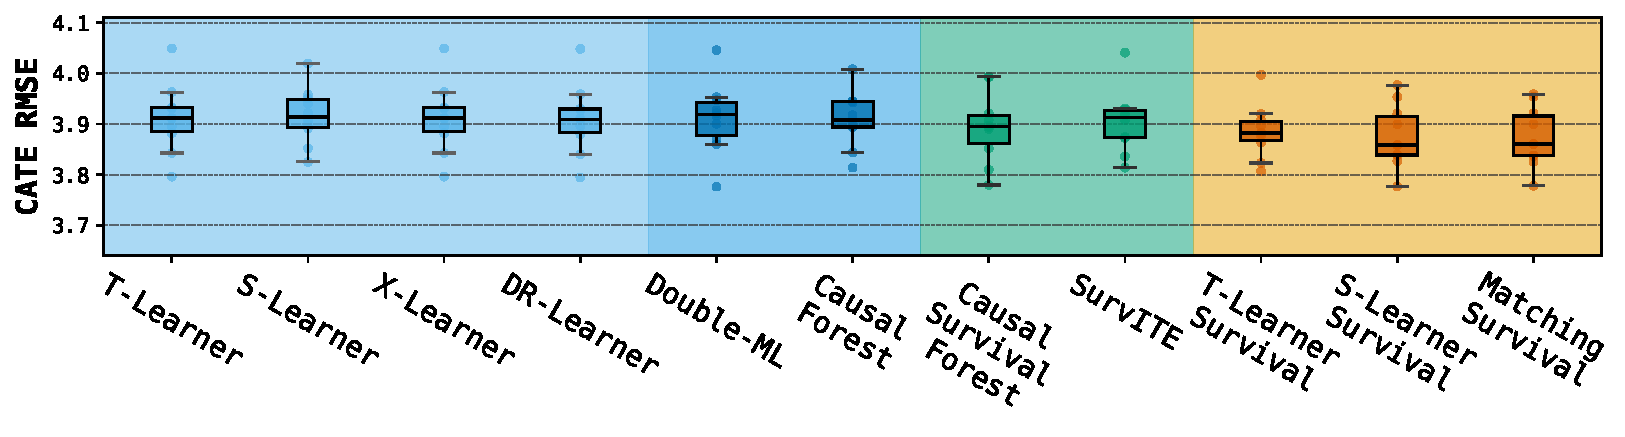
\includegraphics[width=\linewidth]{Chapters/chapter-04/images/figure_results_updated/cate_rmse/Scenario_C_OBS-UConf-IC_cate_mse.pdf}
            
            \label{ch04:fig:cate_rmse_scenario_C_OBS_UConf_InfC}
        \end{minipage}} &
        \subfloat[{RCT:\ChFourBlackCross, Ignorability:\ChFourGrayCheck, Positivity:\ChFourBlackCross, Ignorable Censoring:\ChFourBlackCross}]{\begin{minipage}[t]{0.495\textwidth}
            \centering
            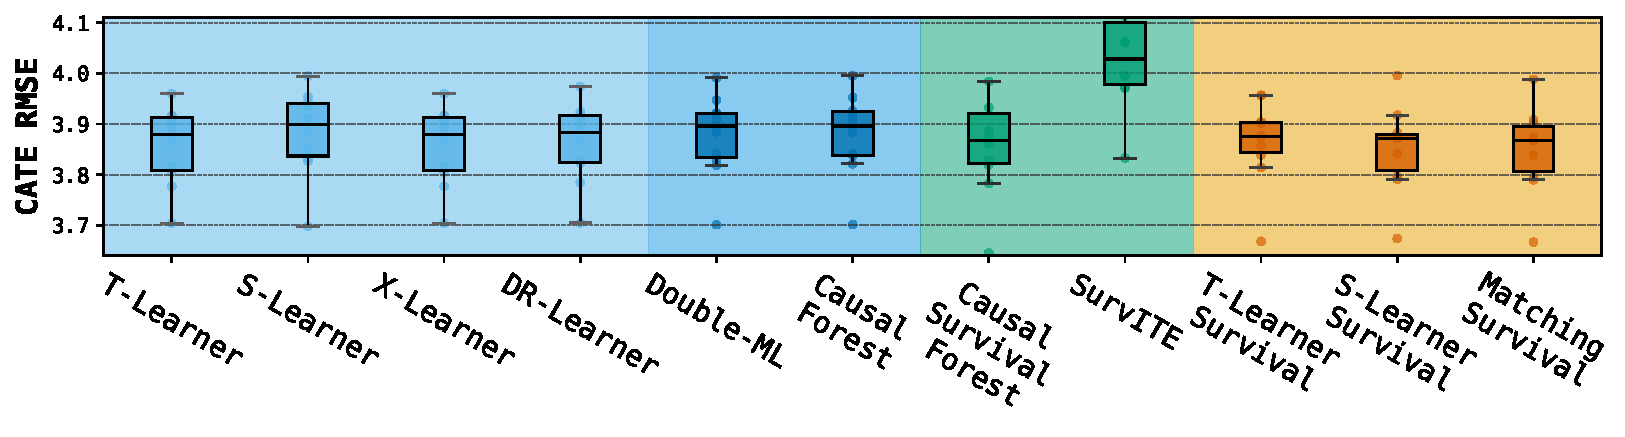
\includegraphics[width=\linewidth]{Chapters/chapter-04/images/figure_results_updated/cate_rmse/Scenario_C_OBS-NoPos-IC_cate_mse.pdf}
            
            \label{ch04:fig:cate_rmse_scenario_C_OBS_NoPos_InfC}
        \end{minipage}}
    \end{tabular}
    }%
    
    
}
\end{figure}


\textbf{Key findings.}
Overall, performance is strongly context-dependent.
For example, in low-censoring randomized settings, outcome imputation methods such as X-Learner and Double-ML excel.
As censoring intensifies or when assumptions are violated, survival meta-learners and Causal Survival Forests gain a clear advantage.
Within method families, the choice of imputation algorithm or survival base model critically determines outcomes. 
Appendix~\ref{ch04:app:additional_synthetic_exps} further supports this pattern quantitatively through Top-$k$ frequency summaries of CATE RMSE and ATE Bias (Tables~\ref{ch04:tab:overall-winrate}-~\ref{ch04:tab:winrate-obs-configs}), highlighting methods that consistently rank at the top rather than merely performing well on average.
% Aggregate win-rate analyses further reinforce this observed pattern, demonstrating that survival-aware method families consistently dominate the top performance (Appendix~\ref{ch04:app:additional_synthetic_exps}). 
We summarize detailed findings below.
% \ChFourRebuttal{Appendix~\ref{ch04:app:additional_synthetic_exps} complements these averages with Top-$k$ frequency summaries across both CATE RMSE and ATE Bias (Tables~\ref{ch04:tab:overall-winrate} ), helping distinguish methods that rank well on average from those that do so consistently.}

\textbf{Overall performance (Q1).}  Figure~\ref{ch04:fig:average_rank_all} (top) presents Borda count rankings of the top-10 performing methods out of the \ChFourRebuttal{53} total configurations evaluated (full ranking in Appendix~\ref{ch04:app:full-rankings}). 
% This analysis reveals a clear advantage for survival meta-learners using DeepSurv as their base model, with Matching-Survival (DeepSurv) ranking first (average rank of 6.70 out of 52) and S-Learner-Survival (DeepSurv) ranking second (6.85). Double-ML with Margin imputation follows closely (7.47), indicating its effectiveness when paired with the right imputation method. 
The highest-performing estimators are survival meta-learners built on DeepSurv, with S-Learner-Survival (average rank 5.17 across \ChFourRebuttal{53} methods) and Matching-Survival (5.42) leading, followed by Double-ML with Margin imputation (6.65). 
Among outcome imputation approaches, Margin appears most frequently among the top performers, though Pseudo-obs and IPCW-T are also represented. 
% Similarly, while Lasso appears more frequently as the base regression model in top-ranked methods (particularly in X-Learner configurations), Random Forest also shows strong performance in certain combinations.
% It is worth nothing that on average across all 40 datasets, more sophisticated outcome imputation approaches, specifically X-Learner and Double-ML, appear multiple times in the top 10, while their simpler counterparts (S-Learner and T-Learner with imputation) are absent from the top ranks. This suggests that more complex meta-learning structures provide substantial benefits when handling censored data through imputation. 
% Causal Survival Forests ranks sixth (12.88), offering competitive performance without requiring method-specific tuning of base models or imputation approaches. All top 10 methods represent strong performers across our comprehensive benchmark, with each demonstrating strengths in different settings as revealed by our more detailed analyses.

At the method family level (Figure~\ref{ch04:fig:cate_mse_scenario_C_main} for Scenario \texttt{C} and Figure~\ref{ch04:fig:average_rank_all} (bottom) across all causal configurations and survival scenarios), we see how each approach performs when optimally configured.
At this level, S-Learner-Survival (average rank \ChFourRebuttal{3.30 across 11 method families}) and Matching-Survival (3.48) maintain their advantage, followed by Double-ML (3.98) and Causal Survival Forests (5.10).
% Complementary win-rate analysis also highlights that Matching-Survival and S-Learner-Survival achieve the most consistent Top-5 placements across all causal and survival conditions (Appendix~\ref{ch04:app:full-rankings}).
%Causal Survival Forests (4.83) ranks fifth, ahead of both Causal Forest (6.40) and T-Learner-Survival (6.47). We can see that standard S-Learner with imputation ranks last (8.07), which highlights that simpler meta-learners paired with an imputation method struggle to compete with more sophisticated approaches in the survival setting.


\textbf{Violations of causal assumptions (Q2).}
Performance shifts substantially depending on assumption violations (Figure~\ref{ch04:fig:average_rank_per_experiments}).
In randomized balanced trials (\texttt{RCT-50}), outcome imputation methods dominate, with Double-ML (3.60) and Causal Forest (5.60) showing performance comparable to high-ranking survival meta-learners.
However, under imbalanced treatment (\texttt{RCT-5}), Double-ML remains strong (1.80), while T-Learner-Survival---which relies on fitting base models on treated units---drops to last place (9.00), alongside SurvITE, due to sparsity of treated samples.
% As we introduce various assumption violations, survival meta-learners increasingly dominate, particularly in scenarios with multiple simultaneous violations like unmeasured confounding with informative censoring (Figure~\ref{ch04:fig:average_rank_per_experiments}(g)), where S-Learner-Survival (2.40) and Causal Survival Forests (3.00) substantially outperform all outcome imputation methods.

Under ignorability violation (\texttt{OBS-UConf}, Figure~\ref{ch04:fig:borda_ranking_causal_config_OBS_UConf}), Double-ML and X-Learner are the main competitive imputation methods, whereas survival meta-learners retain relatively stable performance. 
\textcolor{black}{Examining ATE bias (Figures~\ref{ch04:fig:ate_bias_grid_scenario_A}d-\ref{ch04:fig:ate_bias_grid_scenario_E}d), we see that across all scenarios, survival meta-learners and Causal Survival Forests methods maintain relatively consistent bias levels despite ignorability violations, whereas meta-learners exhibit a slightly increased bias at times.} %This suggest that inherently survival methods may better accommodate unmeasured confounding, possibly because their direct modeling of the survival process captures important structural relationships that help mitigate bias from unobserved factors.
\ChFourRebuttal{This stability is also reflected in aggregated win-rate summaries for \texttt{OBS-UConf}, where survival-aware families most consistently appear among the Top-$k$ for both CATE RMSE and ATE Bias (Appendix~\ref{ch04:app:more-avg-rank}, Table~\ref{ch04:tab:winrate-obs-configs}).}

Under positivity violation (\texttt{OBS-NoPos}, Figure \ref{ch04:fig:borda_ranking_causal_config_OBS_NoPos}), we see the more sophisticated outcome imputation approaches like Double-ML and X-Learner maintain strong performance and outperform survival meta-learners.
However, when positivity violations occur alongside other violations (Figure~\ref{ch04:fig:borda_ranking_causal_config_OBS_NoPos_InfC}), survival meta-learners regain their advantage, demonstrating their robustness to multiple simultaneous violations.
This behavior is also reflected in the win-rate summaries, which show a similar shift in Top-$k$ coverage across configurations (Appendix~\ref{ch04:app:more-avg-rank}, Table~\ref{ch04:tab:winrate-obs-configs}).
Additionally, Causal Survival Forests sees a large drop in its ranking when faced with only positivity violation, suggesting its limited robustness to regions of covariate space with deterministic treatment assignment.

Under informative censoring (\texttt{InfC}, Figure~\ref{ch04:fig:cate_rmse_scenario_C_OBS_CPS_InfC}-~\ref{ch04:fig:cate_rmse_scenario_C_OBS_NoPos_InfC}), survival meta-learners and Causal Survival Forest continue to outperform outcome imputation approaches.
However, all methods show degraded performance compared to their ignorable censoring counterparts, with substantially higher CATE RMSE variability, indicating the increased difficulty of estimation under dependent censoring.

\textbf{Impact of censoring rate (Q3).}
For the impact of censoring rate and survival time distribution (Figure~\ref{ch04:fig:average_rank_per_scenario}), in low-censoring Scenarios \texttt{A} and \texttt{B}, Double-ML leads the rankings, but as censoring increases through Scenarios \texttt{C} to \texttt{E}, survival meta-learners and Causal Survival Forests progressively move to the top.
By Scenario \texttt{D} (high censoring), S-Learner-Survival (1.6) and Matching-Survival (2.4) dramatically outperform all other approaches.
This pattern suggests that direct survival modeling provides increasing advantages as censoring rates rise, likely due to better handling of the uncertainty in heavily censored data compared to outcome imputation approaches.
The same monotonic shift toward survival-aware methods with increasing censoring is visible in their Top-$k$ win-rate coverage across scenarios (Appendix~\ref{ch04:app:average_rank_per_scenario}).

\textcolor{black}{
Separately, in Appendix~\ref{ch04:app:more-ate-plots}, we show ATE bias across different datasets.
We observe apparent divergence of the estimated ATE from the true ATE in Scenario \texttt{D} and slightly in Scenario \texttt{E} (Figure~\ref{ch04:fig:ate_bias_grid_scenario_D}, \ref{ch04:fig:ate_bias_grid_scenario_E}), where the censoring rate is very high. Especially when the true underlying event time follows an AFT distribution (Scenario \texttt{D}), almost all estimators failed under all different causal configurations, suggesting the challenging task of treatment effect estimation under a high censoring rate.
}


% A series of auxiliary evaluation on the imputation and base learner:
% We assess imputation accuracy Appendix~\ref{ch04:subapp:impute-eval}, where Table~\ref{tab:impute-eval} reports the MAE for three candidate methods across different datasets. survival accuracy and base regression accuracy. These will help us under the perforamnce of them on final CATE estimations.


\textbf{Component effects on CATE estimation (Q4).} 
Auxiliary evaluations in Appendix~\ref{ch04:app:auxiliary-eval-results} demonstrate that both imputation accuracy and base learner performance influence downstream CATE estimation.
Among outcome imputation methods, Margin consistently achieves the lowest imputation error and degrades the least under heavy censoring (Appendix~\ref{ch04:subapp:impute-eval}), which translates into Margin-based variants appearing more frequently among the top-ranked estimators (Figure~\ref{ch04:fig:average_rank_all}).
For survival meta-learners, higher concordance indices of DeepSurv across survival scenarios (Appendix~\ref{ch04:subapp:base-surv-eval}) explain why DeepSurv-based configurations dominate overall rankings. 


